\documentclass[10pt,a4paperpaper,openright]{book}
\usepackage{lmodern}
\usepackage{amssymb,amsmath}
\usepackage{ifxetex,ifluatex}
\usepackage{fixltx2e} % provides \textsubscript
\ifnum 0\ifxetex 1\fi\ifluatex 1\fi=0 % if pdftex
  \usepackage[T1]{fontenc}
  \usepackage[utf8]{inputenc}
\else % if luatex or xelatex
  \ifxetex
    \usepackage{mathspec}
  \else
    \usepackage{fontspec}
  \fi
  \defaultfontfeatures{Ligatures=TeX,Scale=MatchLowercase}
\fi
% use upquote if available, for straight quotes in verbatim environments
\IfFileExists{upquote.sty}{\usepackage{upquote}}{}
% use microtype if available
\IfFileExists{microtype.sty}{%
\usepackage{microtype}
\UseMicrotypeSet[protrusion]{basicmath} % disable protrusion for tt fonts
}{}
\usepackage[unicode=true]{hyperref}
\hypersetup{
            pdfborder={0 0 0},
            breaklinks=true}
\urlstyle{same}  % don't use monospace font for urls
\usepackage{graphicx,grffile}
\makeatletter
\def\maxwidth{\ifdim\Gin@nat@width>\linewidth\linewidth\else\Gin@nat@width\fi}
\def\maxheight{\ifdim\Gin@nat@height>\textheight\textheight\else\Gin@nat@height\fi}
\makeatother
% Scale images if necessary, so that they will not overflow the page
% margins by default, and it is still possible to overwrite the defaults
% using explicit options in \includegraphics[width, height, ...]{}
\setkeys{Gin}{width=\maxwidth,height=\maxheight,keepaspectratio}
\IfFileExists{parskip.sty}{%
\usepackage{parskip}
}{% else
\setlength{\parindent}{0pt}
\setlength{\parskip}{6pt plus 2pt minus 1pt}
}
\setlength{\emergencystretch}{3em}  % prevent overfull lines
\providecommand{\tightlist}{%
  \setlength{\itemsep}{0pt}\setlength{\parskip}{0pt}}
\setcounter{secnumdepth}{5}
% Redefines (sub)paragraphs to behave more like sections
\ifx\paragraph\undefined\else
\let\oldparagraph\paragraph
\renewcommand{\paragraph}[1]{\oldparagraph{#1}\mbox{}}
\fi
\ifx\subparagraph\undefined\else
\let\oldsubparagraph\subparagraph
\renewcommand{\subparagraph}[1]{\oldsubparagraph{#1}\mbox{}}
\fi

% set default figure placement to htbp
\makeatletter
\def\fps@figure{htbp}
\makeatother

% Table of contents formatting
\renewcommand{\contentsname}{Table of Contents}
\setcounter{tocdepth}{3}

\setcounter{secnumdepth}{4}


% \renewcommand\thesection{\Roman{section}}

 
% Headers and page numbering 
\usepackage{fancyhdr}

\fancyhead{}
\fancyhead[R]{\leftmark}
\renewcommand{\headrulewidth}{0.4pt}

\fancyfoot[R]{\thepage}
\fancyfoot[C]{}
\fancyfoot[L]{\textit{An Introduction to Symfony 3 \copyright Matt Smith 2017}}
\renewcommand{\footrulewidth}{0.4pt}

\pagestyle{fancy}

% Fonts and typesetting
\setsansfont{Verdana}

% Set figure legends and captions to be smaller sized sans serif font
\usepackage[font={footnotesize,sf}]{caption}

\usepackage{siunitx}

% Adjust spacing between lines to 1.5
\usepackage{setspace}
\onehalfspacing
\raggedbottom

% Set margins
\usepackage[top=1.25in,bottom=1.25in]{geometry}

% Chapter styling
\usepackage[grey]{quotchap}
\makeatletter
\renewcommand*{\chapnumfont}{%
  \usefont{T1}{\@defaultcnfont}{b}{n}\fontsize{80}{100}\selectfont% Default: 100/130
  \color{chaptergrey}%
}
\makeatother

% Set colour of links to black so that they don't show up when printed
\usepackage{hyperref}
\hypersetup{colorlinks=true, linkcolor=black}

% Tables
\usepackage{booktabs}
\usepackage{threeparttable}
\usepackage{array}
\newcolumntype{x}[1]{%
>{\centering\arraybackslash}m{#1}}%

% Allow for long captions and float captions on opposite page of figures 
\usepackage[rightFloats, CaptionBefore]{fltpage}

% Don't let floats cross subsections
\usepackage[section,subsection]{extraplaceins}

\date{}

\begin{document}

\begin{titlepage}
    \begin{center}
    
        \vspace*{1cm}
        

       \large{ \textbf{ \uppercase{An Introduction to Symfony 3}\\(for people that already know OO-PHP and some MVC stuff)}}
        
        \vspace{1.5cm}

        by\\
        \textbf{
        Dr. Matt Smith\\mattsmithdev.com\\goryngge.com\\https://github.com/dr-matt-smith
        }

       

        
        
        \vfill
  
            2017

     \end{center}
    \thispagestyle{empty}
\end{titlepage}

\newpage

\thispagestyle{empty} \mbox{}

\frontmatter

\chapter{Acknowledgements}

Thanks to \ldots{} \tableofcontents

\mainmatter

\part{Introduction to Symfony}

\chapter{Project Introduction}\label{project-introduction}

\section{Project Objectives}\label{project-objectives}

The main goal of this project was to create a simple multi-player based
party game in the Unity video game engine, akin to Mario Party for
example. The game has to have entertainment value. Have simple rules, be
easy to follow and must be capable of being completed, the game must not
be too difficult. The main goals for the game are as follows - There are
a minimum of three players. - One player controls an antagonist type
character represented by a series of fire balls. These fireballs are
lined up horizontally and vertically. - The fireballs lined up
vertically can only move from left to right, and the the fireballs lined
up horizontally can only move up and down. - Two or more players control
the protagonist characters. It is their job to each try and survive the
level for 60 seconds. - It is the player controlling the antagonist's
role to move the fireballs around in an attempt to kill the protagonist
players. - While it is the protagonists job to avoid these fireballs
while also attempting to hinder the other player(s). - There are pickups
which can be collected at certain intervals throughout the level. - One
pickup is a shield which provides the player with invincibility for a
short period of time from the fireballs. - One pickup is a ice blast,
which when picked up adds to an inventory and is used as a projectile to
freeze the other player in place. - There are two game over screens. One
which displays when all protagonist are killed, and another which
displays when a protagonist(s) survive for 60 seconds.

See Figure \ref{image1} for a screenshot.

\begin{figure}
\centering
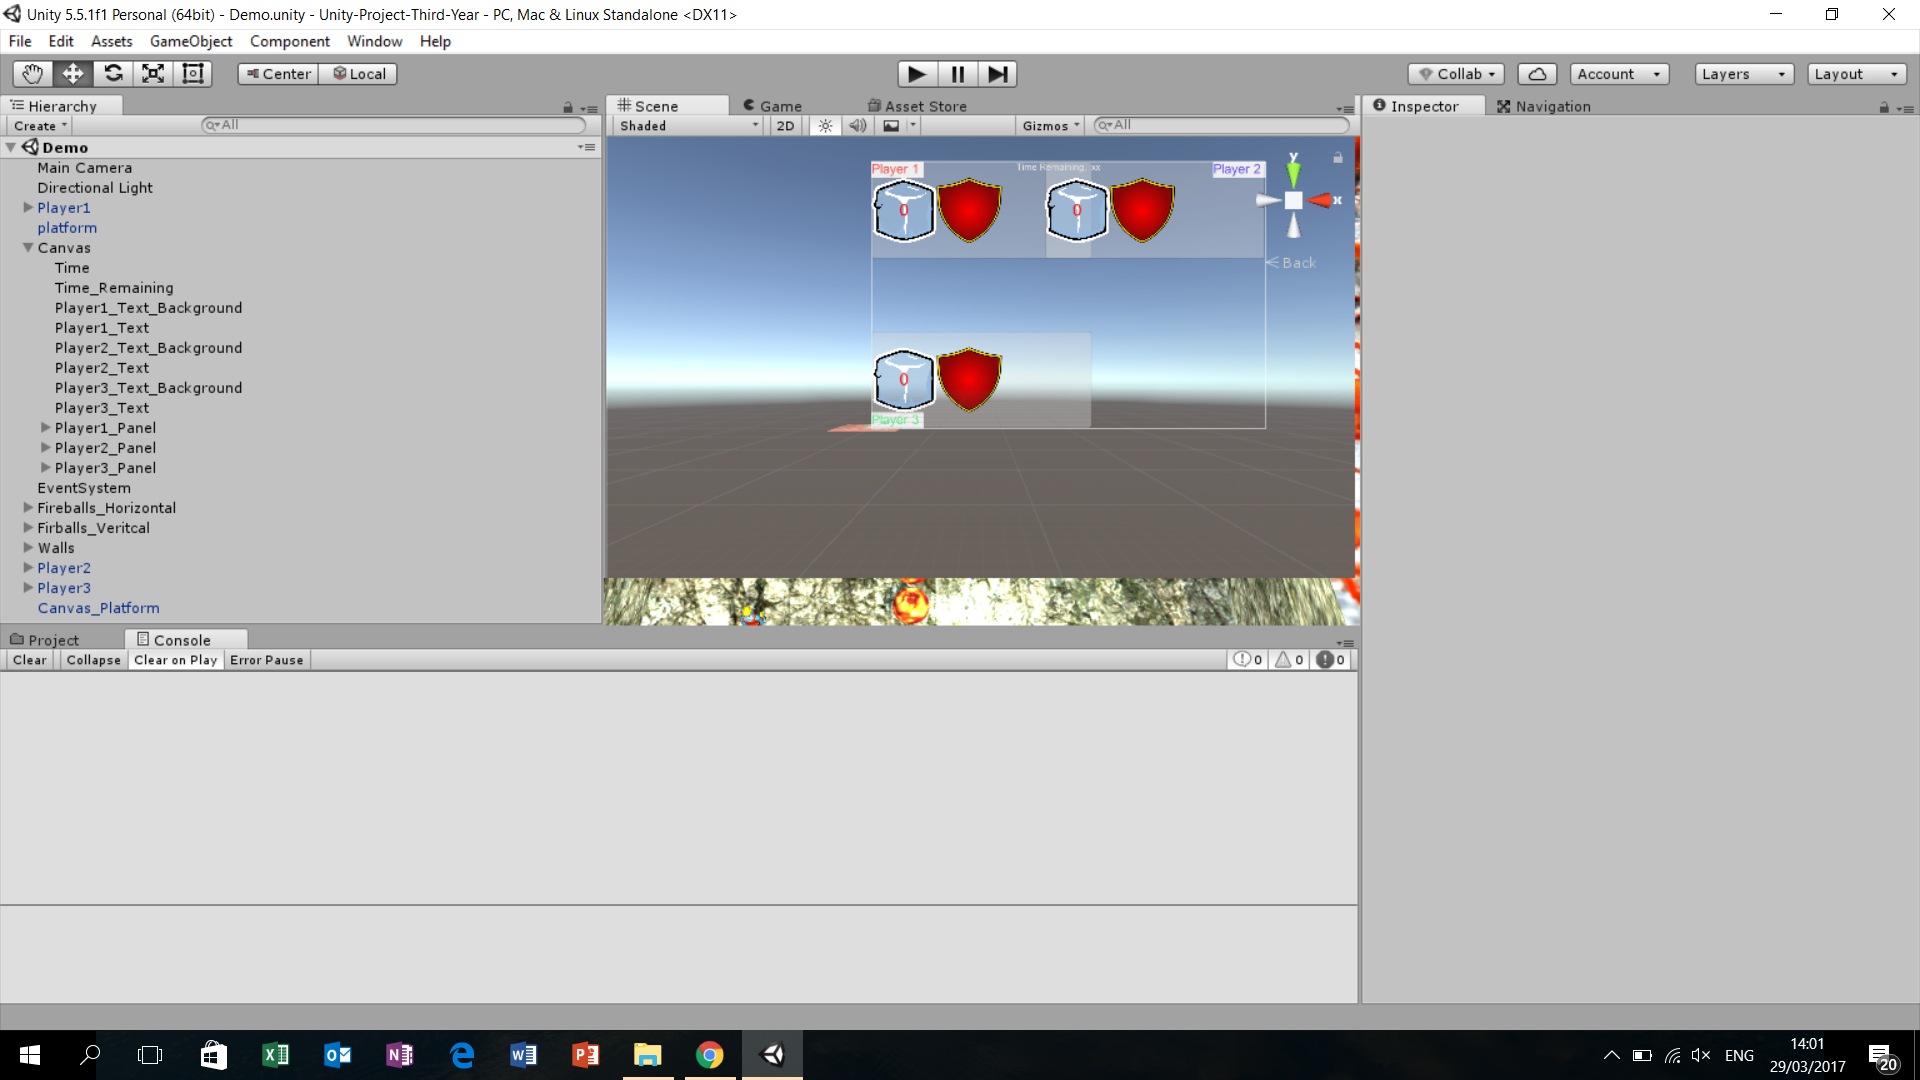
\includegraphics{./03_figures/chapter01/Image1.png}
\caption{A screenshot. \label{image1}}
\end{figure}

\section{Overview of Project}\label{overview-of-project}

For the third year project I decided to develop a game within the Unity
engine that would have multi-player elements to it. When the game was
completed it would be tested within the engine using Xbox controllers
and the keyboard on the PC itself.

The game consists of a minimum of 3 players, one player controlling the
antagonist represented by a series of fireballs, and at least two
players controlling the protagonists consisting of the ``Gravity Guys''.
The two players try so survive the level, while also hindering the other
players with pickups which can be collected throughout the level.

The project was originally supposed to be a group project, it eventually
became an individual project. The project started out as a group
deciding what would be the best way to undergo research in how to
develop this game? What type of a game would it be? How could this game
be developed into an easy to play, and most of all, a fun multi-player
experience?

Research was started by looking at the Unity engine itself and previous
games which have been developed in the engine and the capabilities shown
in these games and if it would be possible to implement these features
into the game I was developing. More research was conducted into
multi-player player games in general, such as what makes them fun to
play and how can you and your friends enjoy the experience as much as
possible?

Also looked at was the issues that some of these games had, and how
exactly could they be improved upon in the game that was being developed
for this project. The final game would then hopefully be completed using
the information gathered from the conducted research. A demo of the
project was displayed in December to show how the basics of how the game
would work, with a full working version being finished by the end of
April.

\section{Overview of Report}\label{overview-of-report}

Chapter 2 will contain the research which was conducted into the
development of this game. Chapter 3 will contain an analysis of how the
game works and the features of the game. While in chapter 4 we will look
at the code used to make all of this feasible.

\section{Research Conducted}\label{research-conducted}

\section{Introduction}\label{introduction}

In this chapter I will present all the relevant research relating to the
project that has been conducted. This includes research of the Unity
engine, games developed in the engine and the history of multi-player
video games and why are they so popular.

\section{Unity and Video Game
Engines}\label{unity-and-video-game-engines}

Almost every one on planet earth has probably come into contact with
video games at some point in their life, whether it through playing
them, watching someone else play them or even seeing a movie previously
based off of a video game. Yes, it is impossible to avoid video games on
modern society. But how exactly are video games made? How does what you
interact with on screen from traversing through space, to saving your
princess from castle to castle, to even playing a virtual sport without
ever having to leave your house made possible? It's simple really, these
are all made possible through the software frameworks which are video
game engines. These engines are used to design the video games in which
you play on your consoles, your PCs and even your mobile devices. These
frameworks provide for you, the tools to make your video game such as,
the physics of your game, the animations, the scripting and the AI.
Popular video game engines include the Frostbite engine, the Unreal
engine, and of course the Unity engine.

The Unity Engine was first announced in 2005 originally only to be used
on Mac OS due to its popularity it has since been extended to 27
platforms such as Desktop, Games Consoles, Virtual Reality and even
Smart Tv's. The popularity of the platform increased even more with the
launch of Unity 5 in 2015 with more than 5 billion games developed in
Unity downloaded in the third quarter of 2016 alone, with the technology
being popular among developers more than any other third party game
development software, with developers including the likes of Ubisoft,
Square Enix, Warner Bros, Obsidian and even Coca Cola.

Many popular games in today's gaming culture have been developed in
Unity including the likes of, Slender: The Eight Pages, a popular
survival horror game in which a player must collect eight pages
scattered throughout a map all while avoiding someone who is following
them. 7 Days to Die, another survival horror game set in an open world
where the player must craft and survive in the wilderness while fighting
against zombies. Cities Skylines, a simulator in which the user builds
entire cities and the rules in which the city operates, and recently the
extremely popular mobile game Pokemon GO was developed in Unity, a game
in which you walk around with your phone and then encounter Pokemon and
use the camera in your phone to capture them.

All of this shows that there are many different features in which can be
implemented into games made using thus engine and just how creative a
developer can be when developing a game which is one the goals of my
project was to try make the game as creative as possible.

\section{Multi-Player Video Games}\label{multi-player-video-games}

\backmatter

\chapter{List of References}\label{list-of-references}

\end{document}
